\documentclass[main.tex]{subfiles}
\usepackage[table,xcdraw]{xcolor}
\usepackage{bm}
\usepackage{wallpaper}
\usepackage{booktabs}
\usepackage{array}
\usepackage{ctex}
\usepackage{longtable}
\usepackage{physics}
\usepackage{fancyhdr}
\usepackage{graphicx} % Required for inserting images
\usepackage{float} %指定图片位置
\usepackage{caption}
\usepackage{pdfpages}
\usepackage{color}
\usepackage{rotating}
\usepackage{tabularray}
\usepackage{xeCJK}
\usepackage{verbatim}
\usepackage{type1cm}
\usepackage{tocloft}
\usepackage{multicol}
\usepackage{amssymb}
\usepackage{amsmath}
\usepackage{float}
\usepackage{wrapfig}
\usepackage{diagbox}
\usepackage{multirow}
\usepackage{subfigure}
\usepackage{svg}
\usepackage[hidelinks]{hyperref}
\usepackage[a4paper,left=2.85cm,right=2.85cm,top=2.54cm,bottom=2.54cm]{geometry}
\renewcommand{\normalsize}{\fontsize{14}{16}\selectfont}


\begin{document}
\chapter{静电场}
\section{静电场的标势}
在静电场中,存在关系:
\begin{align}
    \left\{\begin{array}{l}
    \nabla \cdot \boldsymbol{E} = \frac{\rho}{\varepsilon _0}\\
    \nabla \times \boldsymbol{E} = 0\\
    \boldsymbol{e}_n \times (\boldsymbol{E}_2 - \boldsymbol{E}_1) = 0\\
    \boldsymbol{e}_n \cdot (\boldsymbol{D}_2 - \boldsymbol{D}_1) = \sigma _f
    \end{array}\right.
\end{align}

由$\nabla \times \boldsymbol{E} = 0$,我们可以设一个标量$\varphi$使得$\boldsymbol{E} = -\nabla \varphi$以便于我们对电场的描述.将其代入上方第一式得到Poisson方程:
\begin{align}
    \label{poisson}\nabla ^2 \varphi = - \frac{\rho}{\varepsilon _0}
\end{align}

在介质边界,存在关系:
\begin{align}
    &\varphi _1 = \varphi _2\\
    &\varepsilon _2\frac{\partial \varphi_2}{\partial n} - \varepsilon _1\frac{\partial \varphi_1}{\partial n} = -\sigma _f
\end{align}

其中,$\frac{\partial }{\partial n}$是法向上的偏导数,$\sigma$是界面上的自由电荷面密度.

对于导体而言,其静电条件还需满足以下3点:

(1)导体内部无电荷,电荷只能分布在导体表面;

(2)导体内部电场为0;

(3)导体表面上电场必延法线方向.导体表面为等势面,处处电势相等.

\textbf{静电问题的唯一性定理}:设区域$V$内给定自由电荷分布$\rho(\boldsymbol{x})$,在$V$的边界$S$上给定:

(1)电势$\varphi|_s$

(2)电势的法线方向偏导数$\left. \frac{\partial \varphi}{\partial n}\right|_s$

\section{Laplace方程}
导体内部自由电荷密度$\rho = 0$,于是Poisson方程\ref{poisson}化为Laplace方程:
\begin{align}
    \label{laplace}\nabla ^2 \varphi = 0
\end{align}

其通解可以由分离变量法解出。在球坐标系下,Laplace方程的通解为:
\begin{align}
    \label{Laplacejie}\varphi(R,\theta ,\phi) =&\sum_{n,m}^{} (a_{nm}R^n+\frac{b_{nm}}{R^{n+1}})\mathrm{P}_n^m(\mathrm{cos}\ \theta  )\mathrm{cos}\  m\phi\\
    &+\sum_{n,m}^{} (c_{nm}R^n+\frac{d_{nm}}{R^{n+1}})\mathrm{P}_n^m(\mathrm{cos}\ \theta  )\mathrm{sin}\  m\phi
\end{align}

其中$\mathrm{P}_n^m(\mathrm{cos}\ \theta  )$为\textbf{关联Legendre函数}.若该问题中有对称轴,则可以取其为极轴,则通解不依赖$\phi $,通解变为:
\begin{align}
    \varphi(R,\theta ,\phi) =&\sum_{n}^{} (a_{n}R^n+\frac{b_{n}}{R^{n+1}})\mathrm{P}_n(\mathrm{cos}\ \theta  )
\end{align}

$\mathrm{P}_n(\mathrm{cos}\ \theta  )$为\textbf{Legendre函数}.\ $a_n$,$b_n$由边界条件确定.

\section{镜像法}
\subsection{接地无限大平面导体板}
\begin{figure}[h]
    \centering
    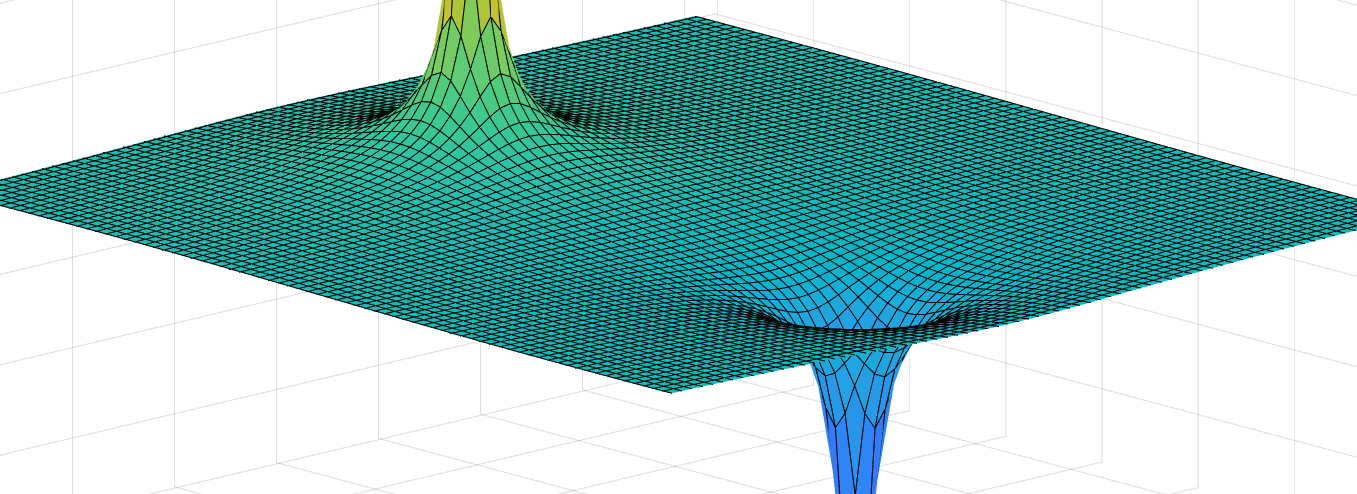
\includegraphics[width=1\linewidth]{jingxiangfa1.png}
\end{figure}

\begin{wrapfigure}{r}{4cm}
	\centering
	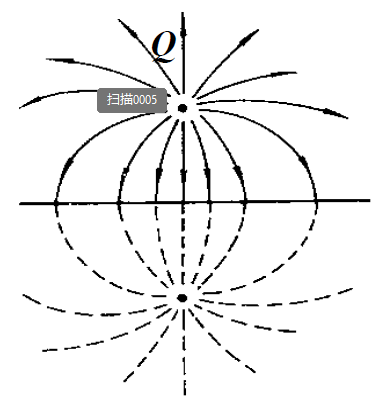
\includegraphics[width=0.9\linewidth]{jingxiangfa2.png}
\end{wrapfigure}

\textbf{例1}\ \ 接地无穷大平面导体板附近有一点电荷$Q$,求空间中的电场.

可以设在导体板下方与$Q$对称位置有一个假想电荷$Q' = -Q$,则空间中任意点$P$点电势为:
\begin{align}
    \varphi(P) = \frac{1}{4\pi \varepsilon _0}\left(\frac{Q}{r} - \frac{Q}{r'} \right)
\end{align}

选$Q$到导体板上的投影点$O$为坐标原点,设$Q$到导体板距离为$a$,则有
\begin{align}
    \varphi (x,y,z) = \frac{1}{4\pi \varepsilon _0}\left[\frac{Q}{\sqrt{x^2+y^2+(z-a)^2}} - \frac{Q}{\sqrt{x^2+y^2+(z+a)^2}} \right]
\end{align}


\subsection{导体球}
\textbf{例2}\ \ 真空中一半径为$R_0$的接地导体球,距球心为$a(a>R_0)$处有一点电荷$Q$,求空间各点的电势.

\begin{figure}[H]
  \centering
  \subfigure{
    \includesvg[width=0.4\linewidth]{jingxiangfa3.svg}}
  \hspace{0.5in} % 两图片之间的距离
  \subfigure{
    \includesvg[width=0.4\linewidth]{jingxiangfa4.svg}}
\end{figure}
可以设在球内有一个假想电荷$Q'$满足关系

\begin{align}
    &b = \frac{R_0^2}{a}\\
    &Q' = -Q\frac{R_0}{a}
\end{align}

这样便可以得到球外任意一点P的电势为

\begin{align}
    \varphi &= \frac{1}{4\pi \varepsilon } \left(\frac{Q}{r} - \frac{R_0Q}{ar'} \right)\nonumber\\
    & = \frac{1}{4\pi \varepsilon } \left(\frac{Q}{\sqrt{R^2+a^2-2Ra\ \mathrm{cos}\ \theta}} - \frac{R_0Q/a}{\sqrt{R^2+b^2-2Rb\ \mathrm{cos}\ \theta}} \right)
\end{align}

\section{多极展开}
对于任意一个电荷体系激发势,我们都可以对其在$\boldsymbol{x}'$处进行多极展开:
\begin{align}
    \varphi(\boldsymbol{x})& = \int_{V}^{} \frac{\rho '(\boldsymbol{x})\mathrm{d}V'}{4\pi \varepsilon _0r}\\
    & = \frac{1}{4\pi \varepsilon _0}\left ( \frac{q}{R} - \boldsymbol{p} \cdot \nabla \frac{1}{R} + \frac{1}{6}\sum_{i,j}^{} \mathcal{D}_{ij}  \frac{\partial^2}{\partial x_i\partial x_j}\frac{1}{R} +... \right ) 
\end{align}

上式第一项称为\textbf{单极子项},第二项称为\textbf{偶极子项},第三项称为\textbf{四极子项}……将其各自所含的参数$q,\ \boldsymbol{p},\ {\substack{\displaystyle\twoheadrightarrow\atop\displaystyle{\mathcal{D}}\\[0.624em]~}}$写出,我们不难发现:
\begin{align}
    &q = \int_{V}^{} \rho (\boldsymbol{x}')\mathrm{d}V'\\
    &\boldsymbol{p} = \int_{V}^{} \rho (\boldsymbol{x}')\boldsymbol{x}' \mathrm{d}V'\\
    &{\substack{\displaystyle\twoheadrightarrow\atop\displaystyle{\mathcal{D}}\\[0.624em]~}}= 3 \int_{V}^{} \rho (\boldsymbol{x}')\boldsymbol{x}' \boldsymbol{x}' \mathrm{d}V'
\end{align}

\textbf{电四极子只有5个独立分量}(无迹对称张量).


\end{document}